%!TEX TS-program = xelatex
\documentclass[11pt]{article}

\usepackage[english]{babel}

\usepackage{amsmath,amssymb,amsfonts}
\usepackage[utf8]{inputenc}
\usepackage[T1]{fontenc}
\usepackage{stix}
\usepackage[scaled]{helvet}
\usepackage[scaled]{inconsolata}

\usepackage{lastpage}

\usepackage{setspace}

\usepackage{ccicons}

\usepackage[hang,flushmargin]{footmisc}

\usepackage{geometry}

\setlength{\parindent}{0pt}
\setlength{\parskip}{6pt plus 2pt minus 1pt}

\usepackage{fancyhdr}
\renewcommand{\headrulewidth}{0pt}\providecommand{\tightlist}{%
  \setlength{\itemsep}{0pt}\setlength{\parskip}{0pt}}

\makeatletter
\newcounter{tableno}
\newenvironment{tablenos:no-prefix-table-caption}{
  \caption@ifcompatibility{}{
    \let\oldthetable\thetable
    \let\oldtheHtable\theHtable
    \renewcommand{\thetable}{tableno:\thetableno}
    \renewcommand{\theHtable}{tableno:\thetableno}
    \stepcounter{tableno}
    \captionsetup{labelformat=empty}
  }
}{
  \caption@ifcompatibility{}{
    \captionsetup{labelformat=default}
    \let\thetable\oldthetable
    \let\theHtable\oldtheHtable
    \addtocounter{table}{-1}
  }
}
\makeatother

\usepackage{array}
\newcommand{\PreserveBackslash}[1]{\let\temp=\\#1\let\\=\temp}
\let\PBS=\PreserveBackslash

\usepackage[breaklinks=true]{hyperref}
\hypersetup{colorlinks,%
citecolor=blue,%
filecolor=blue,%
linkcolor=blue,%
urlcolor=blue}
\usepackage{url}

\usepackage{caption}
\setcounter{secnumdepth}{0}
\usepackage{cleveref}

\usepackage{graphicx}
\makeatletter
\def\maxwidth{\ifdim\Gin@nat@width>\linewidth\linewidth
\else\Gin@nat@width\fi}
\makeatother
\let\Oldincludegraphics\includegraphics
\renewcommand{\includegraphics}[1]{\Oldincludegraphics[width=\maxwidth]{#1}}

\usepackage{longtable}
\usepackage{booktabs}

\usepackage{color}
\usepackage{fancyvrb}
\newcommand{\VerbBar}{|}
\newcommand{\VERB}{\Verb[commandchars=\\\{\}]}
\DefineVerbatimEnvironment{Highlighting}{Verbatim}{commandchars=\\\{\}}
% Add ',fontsize=\small' for more characters per line
\usepackage{framed}
\definecolor{shadecolor}{RGB}{248,248,248}
\newenvironment{Shaded}{\begin{snugshade}}{\end{snugshade}}
\newcommand{\KeywordTok}[1]{\textcolor[rgb]{0.13,0.29,0.53}{\textbf{#1}}}
\newcommand{\DataTypeTok}[1]{\textcolor[rgb]{0.13,0.29,0.53}{#1}}
\newcommand{\DecValTok}[1]{\textcolor[rgb]{0.00,0.00,0.81}{#1}}
\newcommand{\BaseNTok}[1]{\textcolor[rgb]{0.00,0.00,0.81}{#1}}
\newcommand{\FloatTok}[1]{\textcolor[rgb]{0.00,0.00,0.81}{#1}}
\newcommand{\ConstantTok}[1]{\textcolor[rgb]{0.00,0.00,0.00}{#1}}
\newcommand{\CharTok}[1]{\textcolor[rgb]{0.31,0.60,0.02}{#1}}
\newcommand{\SpecialCharTok}[1]{\textcolor[rgb]{0.00,0.00,0.00}{#1}}
\newcommand{\StringTok}[1]{\textcolor[rgb]{0.31,0.60,0.02}{#1}}
\newcommand{\VerbatimStringTok}[1]{\textcolor[rgb]{0.31,0.60,0.02}{#1}}
\newcommand{\SpecialStringTok}[1]{\textcolor[rgb]{0.31,0.60,0.02}{#1}}
\newcommand{\ImportTok}[1]{#1}
\newcommand{\CommentTok}[1]{\textcolor[rgb]{0.56,0.35,0.01}{\textit{#1}}}
\newcommand{\DocumentationTok}[1]{\textcolor[rgb]{0.56,0.35,0.01}{\textbf{\textit{#1}}}}
\newcommand{\AnnotationTok}[1]{\textcolor[rgb]{0.56,0.35,0.01}{\textbf{\textit{#1}}}}
\newcommand{\CommentVarTok}[1]{\textcolor[rgb]{0.56,0.35,0.01}{\textbf{\textit{#1}}}}
\newcommand{\OtherTok}[1]{\textcolor[rgb]{0.56,0.35,0.01}{#1}}
\newcommand{\FunctionTok}[1]{\textcolor[rgb]{0.00,0.00,0.00}{#1}}
\newcommand{\VariableTok}[1]{\textcolor[rgb]{0.00,0.00,0.00}{#1}}
\newcommand{\ControlFlowTok}[1]{\textcolor[rgb]{0.13,0.29,0.53}{\textbf{#1}}}
\newcommand{\OperatorTok}[1]{\textcolor[rgb]{0.81,0.36,0.00}{\textbf{#1}}}
\newcommand{\BuiltInTok}[1]{#1}
\newcommand{\ExtensionTok}[1]{#1}
\newcommand{\PreprocessorTok}[1]{\textcolor[rgb]{0.56,0.35,0.01}{\textit{#1}}}
\newcommand{\AttributeTok}[1]{\textcolor[rgb]{0.77,0.63,0.00}{#1}}
\newcommand{\RegionMarkerTok}[1]{#1}
\newcommand{\InformationTok}[1]{\textcolor[rgb]{0.56,0.35,0.01}{\textbf{\textit{#1}}}}
\newcommand{\WarningTok}[1]{\textcolor[rgb]{0.56,0.35,0.01}{\textbf{\textit{#1}}}}
\newcommand{\AlertTok}[1]{\textcolor[rgb]{0.94,0.16,0.16}{#1}}
\newcommand{\ErrorTok}[1]{\textcolor[rgb]{0.64,0.00,0.00}{\textbf{#1}}}
\newcommand{\NormalTok}[1]{#1}

\newlength{\cslhangindent}
\setlength{\cslhangindent}{1.5em}
\newlength{\csllabelwidth}
\setlength{\csllabelwidth}{3em}
\newenvironment{CSLReferences}[3] % #1 hanging-ident, #2 entry spacing
 {% don't indent paragraphs
  \setlength{\parindent}{0pt}
  % turn on hanging indent if param 1 is 1
  \ifodd #1 \everypar{\setlength{\hangindent}{\cslhangindent}}\ignorespaces\fi
  % set entry spacing
  \ifnum #2 > 0
  \setlength{\parskip}{#2\baselineskip}
  \fi
 }%
 {}
\usepackage{calc} % for \widthof, \maxof
\newcommand{\CSLBlock}[1]{#1\hfill\break}
\newcommand{\CSLLeftMargin}[1]{\parbox[t]{\maxof{\widthof{#1}}{\csllabelwidth}}{#1}}
\newcommand{\CSLRightInline}[1]{\parbox[t]{\linewidth}{#1}}
\newcommand{\CSLIndent}[1]{\hspace{\cslhangindent}#1}\geometry{verbose,letterpaper,tmargin=2.5cm,bmargin=2.5cm,lmargin=2.5cm,rmargin=4.5cm}

\usepackage{lineno}
\usepackage[nolists,noheads]{endfloat}

\pagestyle{plain}

\doublespacing

\fancypagestyle{normal}
{
  \fancyhf{}
  \fancyfoot[R]{\footnotesize\sffamily\thepage\ of \pageref*{LastPage}}
}
\begin{document}
\thispagestyle{empty}
{\Large\bfseries\sffamily Global knowledge gaps in species interaction
networks data}
\vskip 5em

%
\href{https://orcid.org/0000-0002-0735-5184}{Timothée\,Poisot}%
%
\,\textsuperscript{1,2,‡}\quad %
\href{https://orcid.org/0000-0002-5956-069X}{Gabriel\,Bergeron}%
%
\,\textsuperscript{3}\quad %
\href{https://orcid.org/0000-0001-6619-9874}{Kevin\,Cazelles}%
%
\,\textsuperscript{4,2}\quad %
\href{https://orcid.org/0000-0003-3328-9958}{Tad\,Dallas}%
%
\,\textsuperscript{5}\quad %
\href{https://orcid.org/0000-0002-4498-7076}{Dominique\,Gravel}%
%
\,\textsuperscript{3,2}\quad %
\href{https://orcid.org/0000-0003-1162-169X}{Andrew\,MacDonald}%
%
\,\textsuperscript{1,3}\quad %
\href{https://orcid.org/0000-0002-4104-9463}{Benjamin\,Mercier}%
%
\,\textsuperscript{3}\quad %
\href{https://orcid.org/0000-0001-6217-5891}{Clément\,Violet}%
%
\,\textsuperscript{3}\quad %
\href{https://orcid.org/0000-0002-0866-4376}{Steve\,Vissault}%
%
\,\textsuperscript{3,1,2,‡}

\textsuperscript{1}\,Université de
Montréal\quad \textsuperscript{2}\,Québec Centre for Biodiversity
Sciences\quad \textsuperscript{3}\,Université de
Sherbrooke\quad \textsuperscript{4}\,University of
Guelph\quad \textsuperscript{5}\,Louisiana State University

\textsuperscript{‡}\,These authors contributed equally to the work\\

\textbf{Correspondance to:}\\
Timothée Poisot --- \texttt{timothee.poisot@umontreal.ca}\\

\vfill
This work is released by its authors under a CC-BY 4.0 license\hfill\ccby\\
Last revision: \emph{\today}

\clearpage
\thispagestyle{empty}

\vfill
\textbf{\sffamily Abstract: }Ecological networks are increasingly
studied at large spatial scales, expanding their focus from a conceptual
tool for community ecology into one that also adresses questions in
biogeography and macroecology. This effort is supported by increased
access to standardized information on ecological networks, in the form
of openly accessible databases. Yet, there has been no systematic
evaluation of the fitness for purpose of these data to explore synthesis
questions at very large spatial scales. In particular, because the
sampling of ecological networks is a difficult task, they are likely to
not have a good representation of the diversity of Earth's bioclimatic
conditions, likely to be spatially aggregated, and therefore unlikely to
achieve broad representativeness. In this paper, we analyze over 1300
ecological networks in the mangal.io database, and discuss their
coverage of climates, and the geographic areas in which there is a
deficit of data on ecological networks. Taken together, our results
suggest that while some information about the global structure of
ecological networks is available, it remains fragmented over space, with
further differences by types of ecological interactions. This causes
great concerns both for our ability to transfer knowledge from one
region to the next, but also to forecast the structural change in
networks under climate change.
\vfill

\clearpage
\linenumbers
\pagestyle{normal}

Ecological networks are a useful representation of ecological systems in
which species or organisms interact (Heleno et al. 2014; Delmas et al.
2018). In addition to using the established mathematical framework of
graph theory to describe the structure of species interactions, network
ecology has related the structural and ecological properties of networks
(Proulx, Promislow, and Phillips 2005; Poulin 2010). Networks often
allow to link disconnected scales in ecology (Guimarães 2020), and in
particular are powerful tools to bridge data on populations to ecosystem
properties (Loreau 2010; Jordano and Bascompte 2013; Gonzalez et al.
2020). Recently, the interest in the dynamics of ecological networks
across large temporal scales (Baiser et al. 2019; Tylianakis and Morris
2017), and along environmental gradients (Welti and Joern 2015;
Pellissier et al. 2017; Trøjelsgaard and Olesen 2016), has increased. As
ecosystems are changing rapidly, networks are at risk of undergoing
rapid and catastrophic changes to their structure: for example by
invasion leading to a collapse (Magrach et al. 2017; Strong and Leroux
2014), or by a ``rewiring'' of interactions among existing species (Hui
and Richardson 2019; Guiden et al. 2019; Bartley et al. 2019).
Simulation studies suggest that knowing the structure of the extant
network, \emph{i.e.} being able to map all interactions between species,
is not sufficient (Thompson and Gonzalez 2017) to predict the effects of
external changes; indeed, data on the species occurrences and traits, as
well as local extant and projected climate, are also required.

This change in scope, from describing ecological networks as local,
static objects, to dynamical ones that vary across space and time, has
prompted several methodological efforts. First, tools to study spatial,
temporal, and spatio-temporal variation of ecological networks in
relationship to environmental gradients have been developed and
continuously expanded (Poisot et al. 2012, 2017; Poisot, Stouffer, and
Gravel 2015). Second, there has been an improvement in large-scale
data-collection, through increased adoption of molecular biology tools
(Eitzinger et al. 2019; Evans et al. 2016; Makiola et al. 2019) and
crowd-sourcing of data collection (Bahlai and Landis 2016; Roy et al.
2016; Pocock et al. 2015). Finally, there has been a surge in the
development of tools allowing to \emph{infer} species interactions
(Morales-Castilla et al. 2015; Dallas, Park, and Drake 2017) based on
limited but complementary data on network properties (Stock et al.
2017), species traits (Gravel et al. 2013; Desjardins-Proulx et al.
2017; Brousseau, Gravel, and Tanya Handa 2017; Bartomeus et al. 2016),
and environmental conditions (Gravel et al. 2018). These latter
approaches tend to perform well in data-poor environments (Beauchesne et
al. 2016), and can be combined through ensemble modeling or model
averaging to generate more robust predictions (Pomeranz et al. 2018;
Becker et al. 2020). The task of inferring interactions is particularly
important because ecological networks are difficult to adequately sample
in nature (Jordano 2016a, 2016b; Banašek-Richter, Cattin, and Bersier
2004; Chacoff et al. 2012; Gibson et al. 2011). The common goal to these
efforts is to facilitate the prediction of network structure,
particularly over space (Poisot, Gravel, et al. 2016; Albouy et al.
2019) and into the future (Albouy et al. 2014), to appraise the response
of that structure to possible environmental changes.

These disparate methodological efforts share another important trait:
their continued success at predicting network structure depends both on
state-of-the-art data management, and on the availability of data that
are representative of the area we seek to model. Novel quantitative
tools demand a higher volume of network data; novel collection
techniques demand powerful data repositories; novel inference tools
demand easier integration between different types of data, including but
not limited to: interactions, species traits, taxonomy, occurrences, and
local bioclimatic conditions. Macroecological studies of networks have
demonstrated the importance of integrating network structure with past
and current climate data (Dalsgaard et al. 2013; Schleuning et al. 2014;
Martín-González et al. 2015), and that even when considering large scale
gradients, similar types of interactions can behave in similar ways, in
that they respond to the same drivers (Zanata et al. 2017). That being
said, network-based measures of community structure often bring
complementary information when compared to other sources of data (like
abundance; Dalsgaard et al. 2017).

In short, advancing the science of ecological networks requires us not
only to increase the volume of available data, but also to pair these
data with ecologically relevant metadata. Such data should also be made
available in a way that facilitates programmatic interaction
(\emph{i.e.} where the data are processed automatically and without the
need for manual curation) so that they can be used by reproducible data
analysis pipelines. Poisot, Baiser, et al. (2016) introduced
\texttt{mangal.io} as the first step in this direction. In the years
since the tool was originally published, we continued the development of
data representation, amount and richness of metadata, and digitized and
standardized as much biotic interactions data as we could find. The
second major release of this database contains over 1300 networks,
120000 interactions across close to 7000 taxa, and represents what is to
our best knowledge the most complete collection of species interactions
available.

Here we ask if the current Mangal database is fit for global-scale
synthesis research into ecological networks. A recent study by Cameron
et al. (2019) suggest that food webs are un-evenly documented globally,
but focused on \emph{metadata} as opposed to actual datasets. Here, we
conclude that interactions over most of the planet's surface are poorly
described, despite an increasing amount of available data, due to
temporal and spatial biases in data collection and digitization. In
particular, Africa, South America, and most of Asia have very sparse
coverage. This suggests that synthesis efforts on the worldwide
structure or properties of ecological networks will be weaker within
these areas. To improve this situation, we should digitize available
network information and prioritize sampling towards data-poor locations.

\hypertarget{global-trends-in-ecological-networks-description}{%
\section{Global trends in ecological networks
description}\label{global-trends-in-ecological-networks-description}}

\hypertarget{network-coverage-is-accelerating-but-spatially-aggregated}{%
\subsection{Network coverage is accelerating but spatially
aggregated}\label{network-coverage-is-accelerating-but-spatially-aggregated}}

\begin{figure}
\hypertarget{fig:temporal}{%
\centering
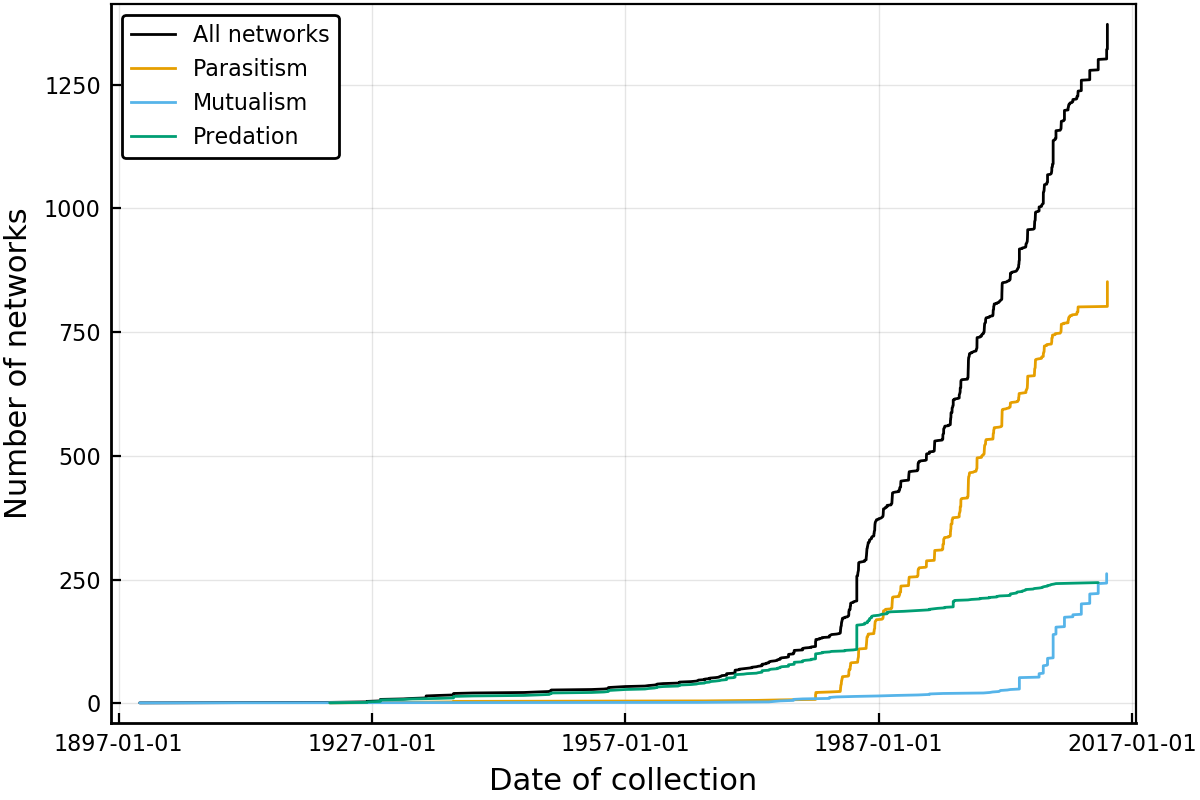
\includegraphics{figures/network_growth_over_time.png}
\caption{Cumulative number of ecological networks available in
\texttt{mangal.io} as a function of the date of collection. About 1000
unique networks have been collected between 1987 and 2017, a rate of
just over 30 networks a year. This temporal increase proceeds at
different rates for different types of networks; while the description
of food webs is more or less constant, the global acceleration in the
dataset is due to increased interest in host-parasite interactions
starting in the late 1970s, while mutualistic networks mostly started
being recorded in the early 2000s.}\label{fig:temporal}
}
\end{figure}

The earliest recorded ecological networks date back to the late
nineteenth century, with a strong increase in the rate of collection
around the 1980s (fig.~\ref{fig:temporal}). Although the volume of
available networks has increased over time, the sampling of these
networks in space has been uneven. In fig.~\ref{fig:spatial}, we show
that globally, network collection is biased towards the Northern
hemisphere, and that different types of interactions have been sampled
in different places. As such, it is very difficult to find a spatial
area of sufficiently large size in which we have networks of predation,
parasitism, and mutualism. The inter-tropical zone is particularly
data-poor, either because data producers from the global South correctly
perceive massive re-use of their data by Western world scientists as a
form of scientific neo-colonialism (as advanced by Mauthner and Parry
2013), thereby providing a powerful incentive \emph{against} their
publication, or because ecological networks are subject to the same data
deficit that is affecting all fields on ecology in the tropics (Collen
et al. 2008). As Bruna (2010) identified almost ten years ago, improved
data deposition requires an infrastructure to ensure they can be
repurposed for future research, which we argue is provided by
\texttt{mangal.io} for ecological interactions.

\begin{figure}
\hypertarget{fig:spatial}{%
\centering
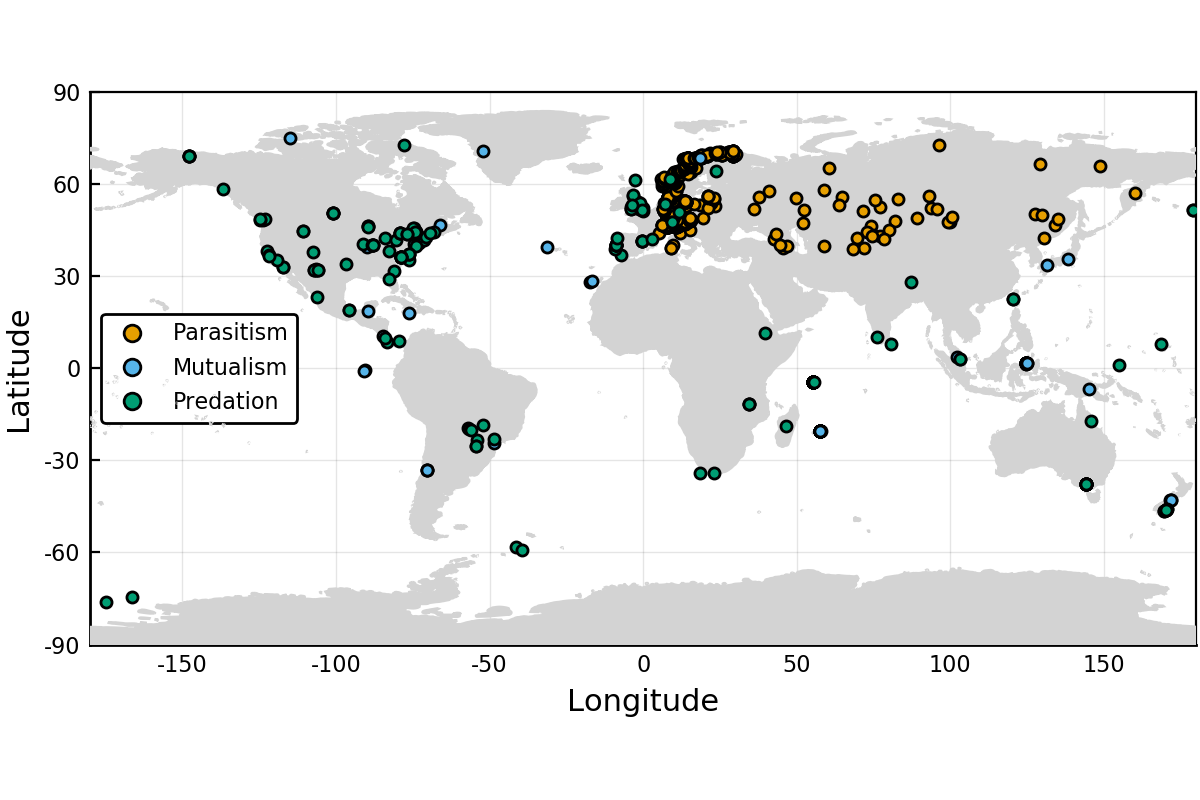
\includegraphics{figures/map_networks_type.png}
\caption{Each point on the map corresponds to a network with parasitic,
mutualistic, and predatory interactions. It is noteworthy that the
spatial coverage of these types of interactions is uneven; the Americas
have almost no recorded parasitic network, for example. Some places have
barely been studied or digitized at all, including Africa and Eastern
Asia. This concentration of networks around rich countries speaks to
inadequate coverage of the diversity of landscapes on
Earth.}\label{fig:spatial}
}
\end{figure}

\hypertarget{network-size-did-not-increase-over-time}{%
\subsection{Network size did not increase over
time}\label{network-size-did-not-increase-over-time}}

In fig.~\ref{fig:size}, we report the changes in the number of nodes
(usually species, sometimes functional or trophic groupings) in
ecological networks over time - interestingly, even though the field of
network ecology itself is growing (Borrett, Moody, and Edelmann 2014),
the overwhelming majority of networks collected to date remain under a
hundred species. This is most likely explained, not by the fact that
ecological networks are necessarily small, but by the immense effort
required to assemble these datasets (Jordano 2016b). Indeed, Jordano
(2016a) emphasizes that the correct empirical description of ecological
networks requires extensive field work in addition to a profound
knowledge of the natural history of the system. These multiple
constraints contribute to keeping network size small, and might not be
indicative of low data quality.

\begin{figure}
\hypertarget{fig:size}{%
\centering
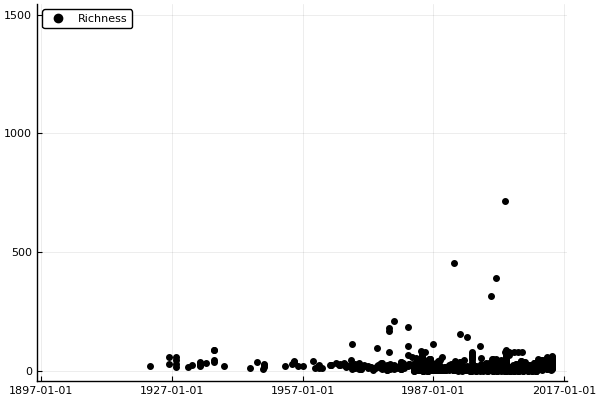
\includegraphics{figures/properties_over_time.png}
\caption{Bins of network size (as measured by the number of nodes)
through time. Although the rythm of network collection has intensified,
most networks that have been archived remain relatively small, most
often having fewer than 100 species.}\label{fig:size}
}
\end{figure}

\hypertarget{different-interaction-types-have-been-studied-in-different-biomes}{%
\subsection{Different interaction types have been studied in different
biomes}\label{different-interaction-types-have-been-studied-in-different-biomes}}

Whittaker (1962) suggested that natural communities can be partitioned
across biomes, largely defined as a function of their relative
precipitation and temperature. For all networks for which the latitude
and longitude were known, we extracted the value temperature (BioClim1,
yearly average) and precipitation (BioClim12, total annual) from the
WorldClim 2 data at a resolution of 10 arc minutes (Fick and Hijmans
2017). Using these we can plot every network on the map of biomes drawn
by Whittaker (1962) (note that because the frontiers between biomes are
not based on any empirical or systematic process, they have been omitted
from this analysis). In fig.~\ref{fig:biomes}, we show that even though
networks capture the overall diversity of precipitation and temperature,
types of networks have been studied in sub-sections of the biomes space
only. Specifically, parasitism networks have been studied in colder and
drier climates; mutualism networks in wetter climates; predation
networks display less of a bias. Interestingly, some combinations of
temperature and precipitation that are abundant on Earth (darker
shading) are not represented in our network dataset, which suggests that
we lack knolwedge of some widespread biomes.

\begin{figure}
\hypertarget{fig:biomes}{%
\centering
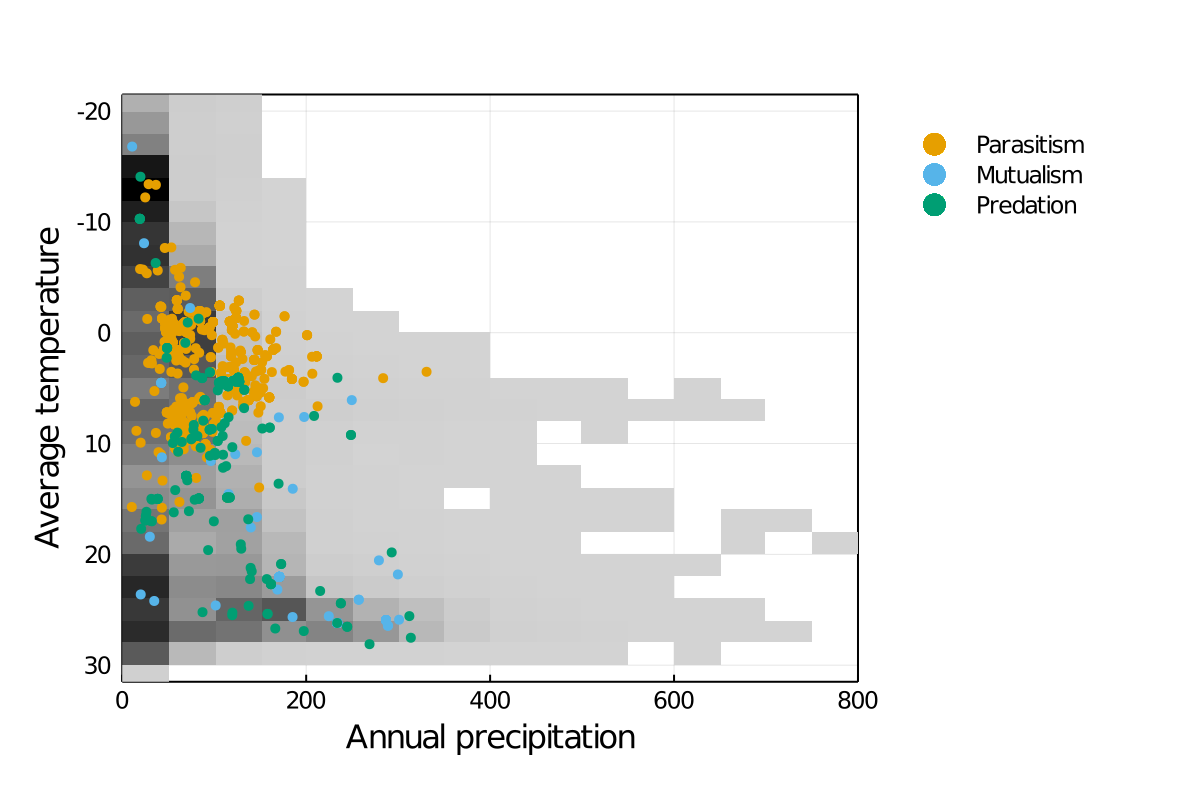
\includegraphics{figures/networks_by_biomes.png}
\caption{List of networks across in the space of biomes as originally
presented by Whittaker (1962). Predation networks, \emph{i.e.} food
webs, seem to have the most global coverage; parasitism networks are
restricted to low temperature and low precipitation biomes, congruent
with the majority of them being in Western Europe. Shading in the
background of the figure represents the relative abundance of the
different precipitation/temperature combinations on Earth, above -60
degrees of latitude.}\label{fig:biomes}
}
\end{figure}

To scale this analysis up to the 19 BioClim variables in Fick and
Hijmans (2017), we extracted the position of every network in the
bioclimatic space, ranged them so that they have mean of 0 and unit
variance, and conducted a principal component analysis on the scaled
bioclimatic variables. In fig.~\ref{fig:pca}, we projected the sampling
locations in the resulting subspace formed by the first two principal
components, which capture well over 75\% of the total variance in the 19
bioclimatic variables. This ordination has a number of interesting
properties. First, the different types of networks occupy different
environmental combinations, which largely matches the results of
fig.~\ref{fig:biomes}. Second, the space is more scarcely sampled by
networks that contain either mostly predatore or mostly mutualistic
interactions -- although they do cover a larger part of the space, the
distance between them is much greater than compared to parasitism.

\begin{figure}
\hypertarget{fig:pca}{%
\centering
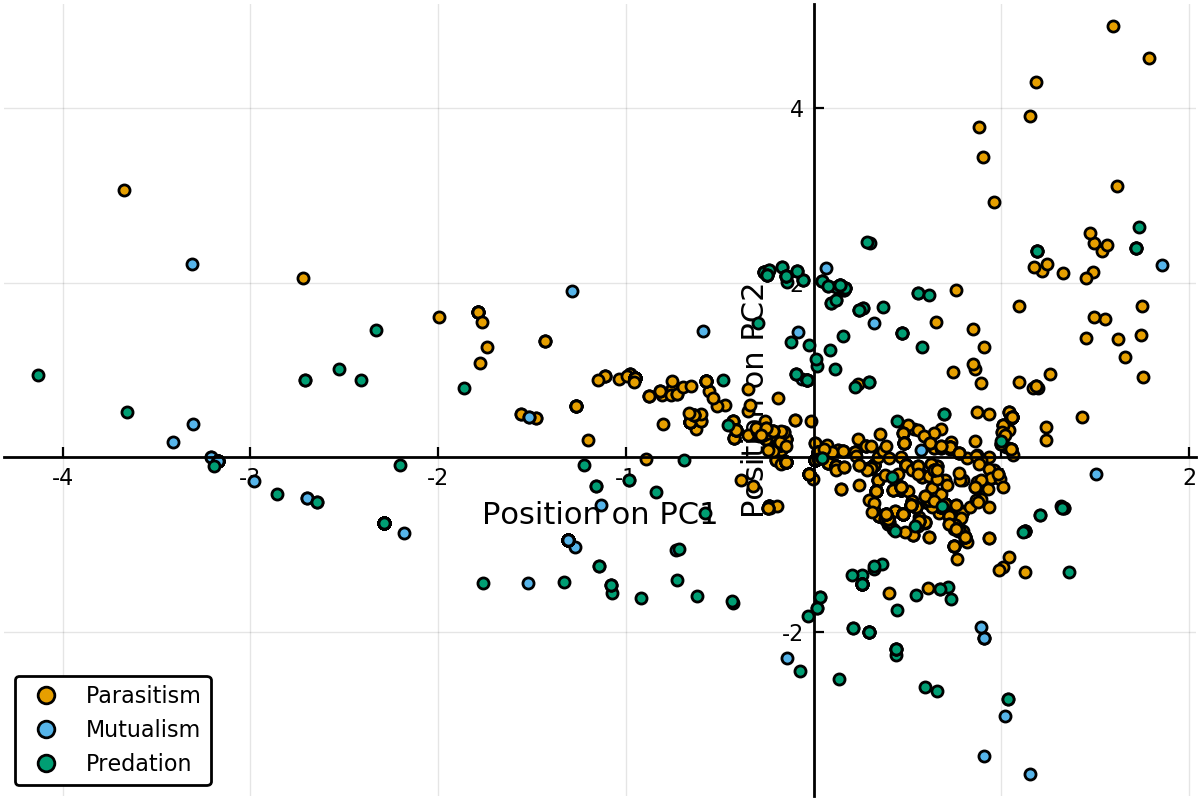
\includegraphics{figures/networks_pca.png}
\caption{Position of the sampled networks on the first two principal
components of the bioclimatic space, as per a principal component
analysis performed and centered and reduced bioclim variables. The first
two axes explain approx. 56\% and 23\% of the total
variance.}\label{fig:pca}
}
\end{figure}

In fig.~\ref{fig:ecc}, we measure the Euclidean distance to the centroid
of the space for every network. Mutualistic interactions tend to have
values that are higher than predation, which are themselves mostly
higher than parasitism. This suggests a potential bias in that globally,
as the growth of digitized ecological networks was largely driven by
parasitic interactions fig.~\ref{fig:temporal}, the environments in
which they have been sampled have became over-represented.

\begin{figure}
\hypertarget{fig:ecc}{%
\centering
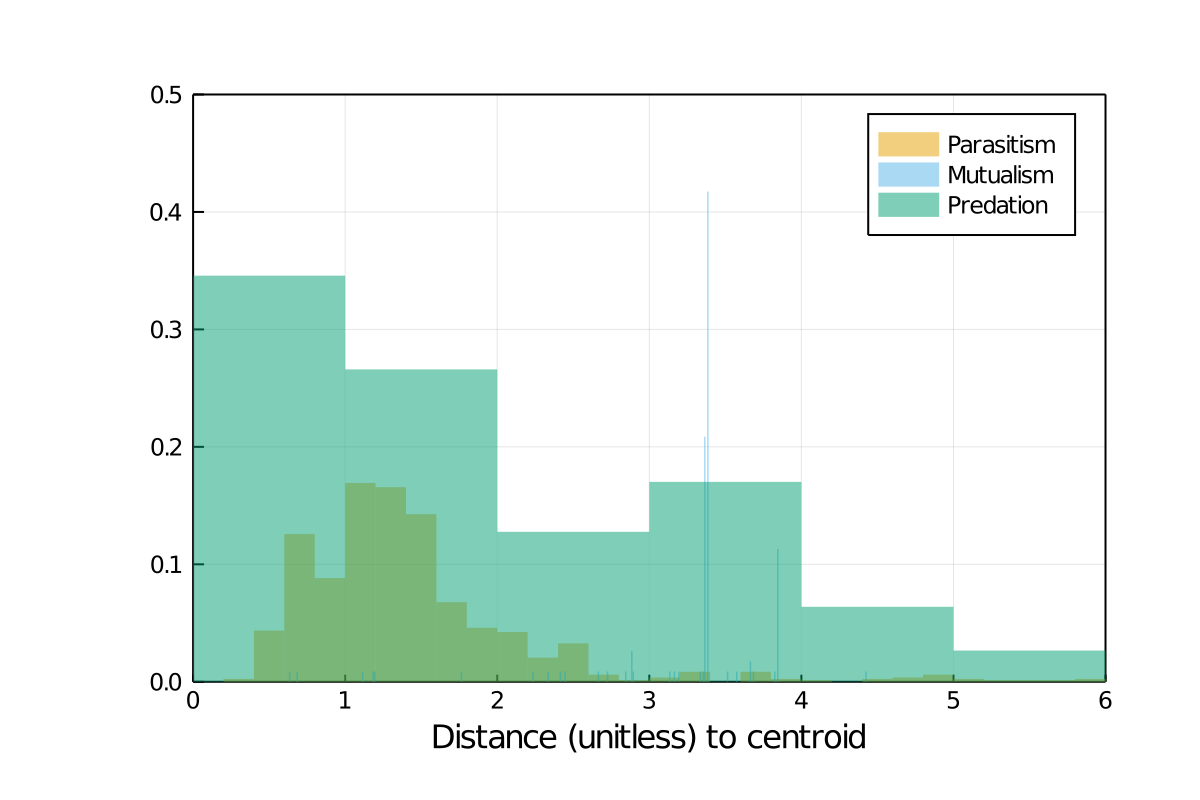
\includegraphics{figures/distance_to_centroid.png}
\caption{Density of the distance to the centroid (in the scaled climatic
space) for each network, by type of interaction. Larger values indicate
that the network is far from its centroid, and therefore represents
sampling in a more ``unique'' location. Mutualistic interactions have
been, on average, studied in more diverse locations that parasitism or
predatory networks.}\label{fig:ecc}
}
\end{figure}

\hypertarget{some-locations-on-earth-have-no-climate-analog}{%
\subsection{Some locations on Earth have no climate
analog}\label{some-locations-on-earth-have-no-climate-analog}}

In figures fig.~\ref{fig:envspace}, we represent the environmental
distance between every pixel covered by \emph{BioClim} data, and the
three networks that were sampled in the closest environmental conditions
(this amounts to a \(k\) nearest neighbors with \(k = 3\)). In short,
higher distances correspond to pixels on Earth for which no climate
analog network exists, whereas the darker areas are well described. It
should be noted that the three types of interactions studied here
(mutualism, parasitism, predation) have regions with no analogs in
different locations. In short, it is not that we are systematically
excluding some areas, but rather than some type of interactions are more
studied in specific environments. This shows how the lack of global
coverage identified in fig.~\ref{fig:biomes}, for example, can cascade
up to the global scale. These maps serve as an interesting measure of
the extent to which spatial predictions can be trusted: any
extrapolation of network structure in an area devoid of analogs should
be taken with much greater caution than an extrapolation in an area with
many similar networks.

\begin{figure}
\hypertarget{fig:envspace}{%
\centering
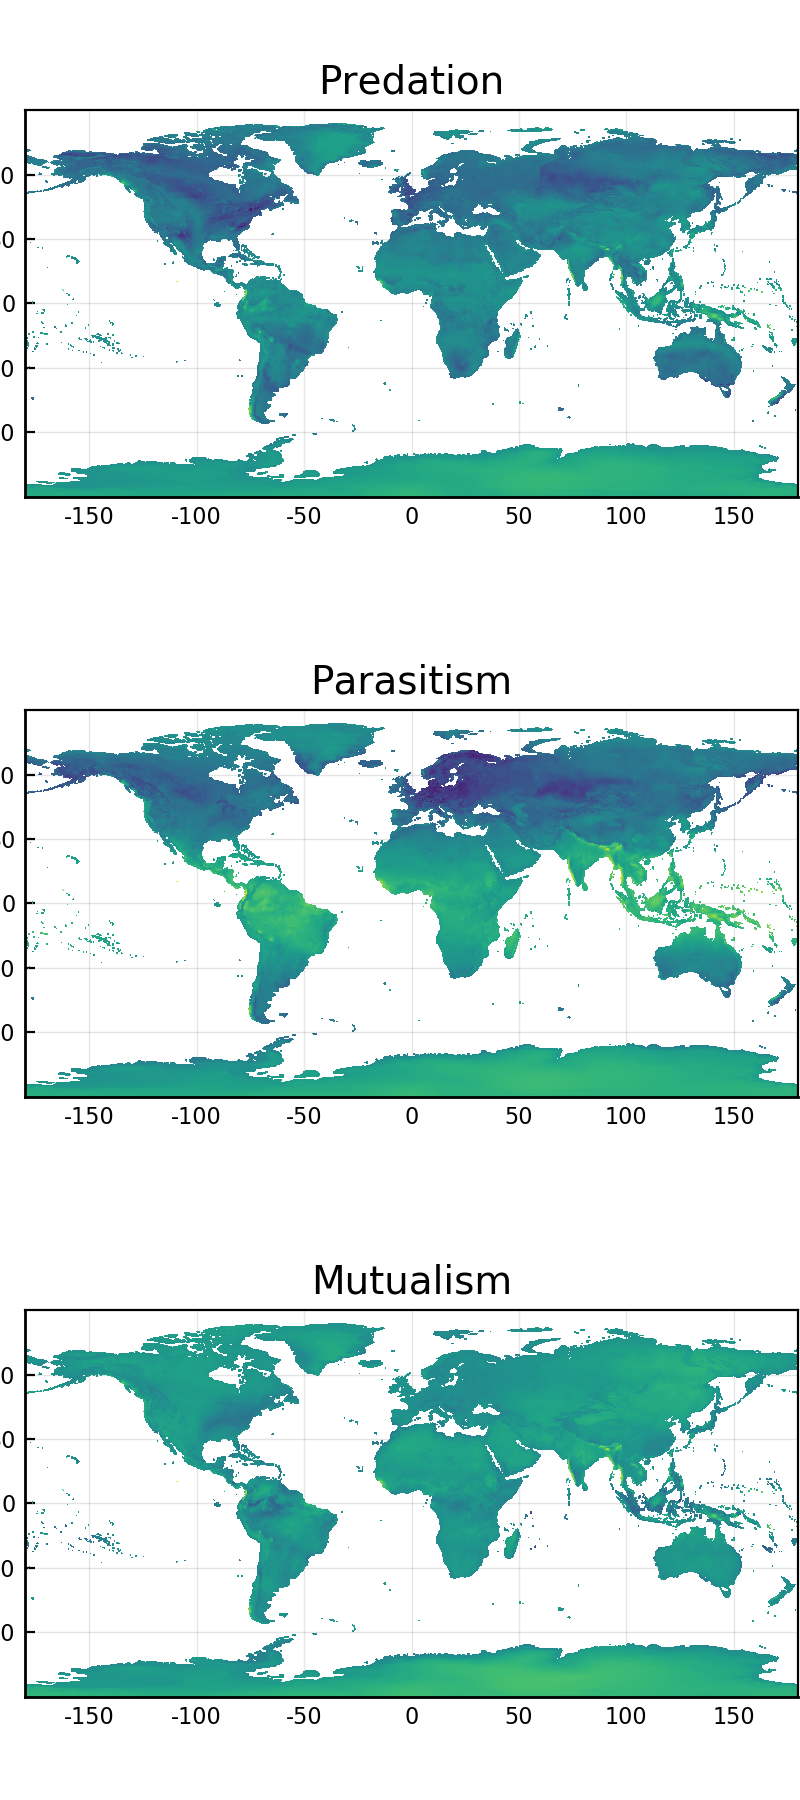
\includegraphics{figures/combined_envirodist_maps.png}
\caption{Environmental distance for every terrestrial pixel to its three
closest networks. Areas of more yellow coloration are further away from
any sampled network, and can therefore not be well predicted based on
existing empirical data. Areas with a dark blue coloration have more
analogs. The distance is expressed in arbitrary units and is
relative.}\label{fig:envspace}
}
\end{figure}

\hypertarget{conclusions}{%
\section{Conclusions}\label{conclusions}}

\hypertarget{for-what-purpose-are-global-ecological-network-data-fit}{%
\subsection{For what purpose are global ecological network data
fit?}\label{for-what-purpose-are-global-ecological-network-data-fit}}

What can we achieve with our current knowledge of ecological networks?
The overview presented here shows a large and detailed dataset, compiled
from almost every major biome on Earth. It also displays our failure as
a community to include some of the most threatened and valuable habitats
in our work. Gaps in any dataset create uncertainty when making
predictions or suggesting causal relationships. This uncertainty must be
measured by users of these data, especially when predicting over the
``gaps'' in space or climate that we have identified. We are not making
any explicit recommendations for synthesis workflows. Rather we argue
that this needs to be a collective process, a collaboration between data
collectors (who understand the deficiencies of these data) and data
analysts (who understand the needs and assumptions of network methods).

One line of research that we feel can confidently be pursued lies in
extrapolating the structure of ecological networks over gradients, not
at the level of species and their interactions, but at that of the
community. Mora et al. (2018) revealed that all food webs are built upon
the same structural backbone, which is in part due to strong
evolutionary constraints on the establishment of species interactions
(Dalla Riva and Stouffer 2015); in other words, most networks are
expected to be variations on a shared theme, and this facilitates the
task of predicting the overarching structure greatly. Finally, this
approach to prediction which neglects the composition of networks is
justified by the observation that network structure tends to be
maintained at very large spatial scales even in the presence of strong
compositional turnover (Dallas and Poisot 2017; Kemp et al. 2017). In
short, the invariance of some network properties allows examining how
``ecological networks'' changes, as abstract objects, over time and
space. One thing that the current state of the data does not always
allow is to examine how a specific group of species (\emph{i.e.} when
taxonomic turnover becomes important) would react, in its interactions,
to environmental gradients. This is an important research question, and
we think that spatially replicated sampling of networks in the future
would help with generating adequate data to address it in a synthetic
way.

\hypertarget{can-we-predict-the-future-of-ecological-networks-under-climate-change}{%
\subsection{Can we predict the future of ecological networks under
climate
change?}\label{can-we-predict-the-future-of-ecological-networks-under-climate-change}}

Perhaps unsurprisingly, most of our knowledge on ecological networks is
derived from data that were collected after the 1990s
(fig.~\ref{fig:temporal}). This means that we have worryingly little
information on ecological networks before the acceleration of the
climate crisis, and therefore lack a robust baseline. Dalsgaard et al.
(2013) provide strong evidence that the extant shape of ecological
networks emerged in part in response to historical trends in climate
change. The lack of reference data before the acceleration of the
effects of climate change is of particular concern, as we may be
deriving intuitions on ecological network structure and assembly rules
from networks that are in the midst of important ecological
disturbances. Although there is some research on the response of
co-occurrence and indirect interactions to climate change (Araújo et al.
2011; Losapio and Schöb 2017), these are a far cry from actual direct
interactions; similarly, the data on ``paleo-foodwebs,'' \emph{i.e.}
from deep evolutionary time (Muscente et al. 2018; Yeakel et al. 2014;
Nenzén, Montoya, and Varela 2014) represent the effect of more
progressive change, and may not adequately inform us about the future of
ecological networks under severe climate change. However, though we lack
baselines against which to measure the present, as a community we are in
a position to provide one for the future. Climate change will continue
to have important impacts on species distributions and interactions for
at least the next century. The Mangal database provides a structure to
organize and share network data, creating a baseline for future attempts
to monitor and adapt to biodiversity change.

Possibly more concerning is the fact that the spatial distribution of
sampled networks shows a clear bias towards the Western world,
specifically Western Europe and the Atlantic coasts of the USA and
Canada (fig.~\ref{fig:spatial}). This problem can be somewhat
circumvented by working on networks sampled in places that are close
analogs of those without direct information (almost all of Africa, most
of South America, a large part of Asia). However,
fig.~\ref{fig:envspace} suggests that this approach will rapidly be
limited: the diversity of bioclimatic combinations on Earth leaves us
with some areas lacking suitable analogs. These regions are expected to
bear the worst of the socio-economical (\emph{e.g.} Indonesia) or
ecological (\emph{e.g.} polar regions) consequences of climate change.
Cameron et al. (2019) reached a similar conclusion by focusing on food
webs, and our analysis suggests that this worrying trend is, in fact,
one that is shared by almost all types of interactions. All things
considered, our current knowledge about the structure of ecological
networks at the global scale leaves us under-prepared to predict their
response to a warming world. From the limited available evidence, we can
assume that ecosystem services supported by species interactions will be
disrupted (Giannini et al. 2017), in part because the mismatch between
interacting species will increase (Damien and Tougeron 2019) alongside
the climatic debt accumulated within interactions (Devictor et al.
2012).

\hypertarget{active-development-and-data-contribution}{%
\subsection{Active development and data
contribution}\label{active-development-and-data-contribution}}

This is an open-source project: all data and all code supporting this
manuscript are available on the Mangal project GitHub organization, and
the figures presented in this manuscript are themselves packaged as a
self-contained analysis which can be run at any time. We hope that the
success of this project will encourage similar efforts within other
parts of the ecological community. Besides, we hope that this project
will encourage the recognition of the contribution that software
creators make to ecological research.

One possible avenue for synthesis work, including the contribution of
new data to Mangal, is the use of these published data to supplement and
extend existing ecological network data. This ``semi-private''
ecological synthesis could begin with new data collected by authors --
for example, a host-parasite network of lake fish in Africa, or a
pollination network of hummingbirds in Brazil. Authors could then extend
their analyses by including a comparison to analogous data made public
in Mangal. Upon the publication of the research paper, the original data
could be uploaded to Mangal. This enables the reproducibility of this
particular published paper. Even more powerfully, it allows us to build
a future of dynamic ecological analyses, wherein analyses are
automatically re-done as more data get added. This would allow a sort of
continuous assessment of proposed ecological relationships in network
structure. This cycle of data discovery and reuse is an example of the
Data Life Cycle (Michener 2015) and represents one way to practice
ecological synthesis.

The idea of continuously updated analyses is very promising. Following
the template laid out by White et al. (2019) and Yenni et al. (2019), it
is feasible to update a series of canonical analyses any time the
database grows, to produce a living, automated synthesis of ecological
networks knowledge. To this end, the Mangal database has been integrated
with \texttt{EcologicalNetworks.jl} (Poisot, Belisle, et al. 2019),
which allows the development of flexible network analysis pipelines. One
immediate target would be to borrow the methodology from Carlson et al.
(2019), and provide an estimate of the sampling effort required to
accurately describe combinations of interaction types and bioclimatic
conditions at various places on Earth, to provide recommendations on
sampling effort allocation. Tightening the integration between
infrastructure, data, and models, contributes to building the capacity
of our field to bring about iterative near-term forecasting of
ecological network structure (Dietze et al. 2018).

\hypertarget{what-problems-would-more-data-solve}{%
\subsection{What problems would more data
solve?}\label{what-problems-would-more-data-solve}}

As the amount of empirical evidence grows, so too should our
understanding of existing relationships between network properties,
between networks properties and space, and the interpretation to be
drawn from them. But what information would the structure of the food
web from a pond bring to our understanding of the plant-pollinator
interactions around it? Or to a food web in another pond a few
kilometers from here? In short, will we get a lot more insights by
accumulating data? Before answering this question (in the affirmative),
it matters to recognize that, as Hortal et al. (2015) pointed out,
biotic interactions are a core part of biodiversity; the Eltonian
shortfall, manifested in our lack of widespread data about them, in as
much of an impediment to our mission as ecologists as the absence of
data on phylogeny or species occurrence would be. As a conclusion to
this article, we would like to frame the aggregation of data on species
interaction networks in standardized databases as both a requirement
justified by fundamental science, and as an opportunity to conduct novel
experiments on the prediction of ecological networks. In fact,
re-analysis of the raw food web data contained in \texttt{mangal.io}
recently allowed MacDonald, Banville, and Poisot (2020) to develop a
novel model of food web structure, which outperforms previous
proposition for the relationship between species richness and link
number.

First, we \emph{require} to collect data on species interactions
following their measurement \emph{in situ} because there is mounting
evidence that they cannot reliably be inferred from observing the two
species in co-occurrence; this has been shown through experimental and
modeling approaches (Barner et al. 2018; Thurman et al. 2019). A recent
synthesis by Blanchet, Cazelles, and Gravel (2020) also reveals how the
assumption that co-occurrence will inform our knowledge of species
interactions as wholly unsupported by the corpus of ecological theories.
With the mounting amount of information on species distribution, and
initiatives like GBIF storing over a billion record of occurrences,
inferring interactions this ways was tempting; sadly, it appears
unfeasible, leaving the curation of interaction data as the justifiable
decision moving forward.

Second, we \emph{should} collect data on species interactions following
their measurement \emph{in situ}, because this will enable the
development of new generation of general models. Initial guidelines by
Morales-Castilla et al. (2015) have led to an increase in the
development and application of forecasting methods (reviewed in the
introduction of this manuscript), and it is now clear that coupling data
on species interaction, occurrences, traits (Schleuning et al. 2020),
phylogeny, is going to lead to powerful predictive models of community
structure. While knowing the structure of the food web of two ponds a
few kilometers apart is not going to qualitatively change our
understanding of food webs as a whole, the accumulation of data about
different interactions in multiple environments will allow us to hunt
for generalities, and identify rules that govern the assemblage of
ecological networks.

Third, we should focus on digitizing, or collecting, time series of
network structure. Networks are known to vary over short (Trøjelsgaard
and Olesen 2016), long (Burkle, Marlin, and Knight 2013), and very long
(Nenzén, Montoya, and Varela 2014) periods of time, and having the
ability to track changes of a network through time will provide
important answers as to the suitability of a single, discrete sampling
timepoint to serve as a reference state for the history of the entire
network. This is of particular relevance as we now have both population
time-series for various community assemblages (Dornelas et al. 2018),
and the quantitative tools to analyse time-series of complex
interactions (Ovaskainen et al. 2017). As of now, very few networks are
\emph{proper} temporal re-sampling of a single site, and this limits our
ability to understand how networks change in nature.

In conclusion, by accumulating more data, we will increase the overlap
between different databases (phylogeny, genetics, occurrences,
functional traits), which will contribute to the unification of our
knowledge of biodiversity, a task which is currently hampered by
disconnectedness between data describing different aspects of community
structure and composition (Poisot, Bruneau, et al. 2019). The work of
predicting species interactions would be streamlined by both (i)
establishing and using a standardized database for species interactions
with contextual metadata, and (ii) ensuring the compatibility of this
database with other sources, through the use of established species
identifiers. The \texttt{mangal} data specification (and database)
solves both issues, and we are confident that through sustained data
deposition, it will contribute to our ability to predict the structure
of ecological networks.

\textbf{Data and code availability:}

All code is available openly at
\texttt{https://github.com/PoisotLab/MangalSamplingStatus}, and the data
can be retrieved from \texttt{mangal.io} and the BioClim database using
the specified files. Also, weekly updated pages presenting the analyses
reported in this manuscript, including the data files, are available at
\texttt{https://poisotlab.github.io/MangalSamplingStatus/}.

\hypertarget{references}{%
\section*{References}\label{references}}
\addcontentsline{toc}{section}{References}

\hypertarget{refs}{}
\begin{CSLReferences}{1}{0}
\leavevmode\hypertarget{ref-Albouy2019MarFis}{}%
Albouy, Camille, Philippe Archambault, Ward Appeltans, Miguel B. Araújo,
David Beauchesne, Kevin Cazelles, Alyssa R. Cirtwill, et al. 2019.
{``The Marine Fish Food Web Is Globally Connected.''} \emph{Nature
Ecology \& Evolution} 3 (8): 1153--61.
\url{https://doi.org/10.1038/s41559-019-0950-y}.

\leavevmode\hypertarget{ref-Albouy2014ProSpe}{}%
Albouy, Camille, Laure Velez, Marta Coll, Francesco Colloca, François Le
Loc'h, David Mouillot, and Dominique Gravel. 2014. {``From Projected
Species Distribution to Food-Web Structure Under Climate Change.''}
\emph{Global Change Biology} 20 (3): 730--41.
\url{https://doi.org/10.1111/gcb.12467}.

\leavevmode\hypertarget{ref-Araujo2011UsiSpe}{}%
Araújo, Miguel B., Alejandro Rozenfeld, Carsten Rahbek, and Pablo A.
Marquet. 2011. {``Using Species Co-Occurrence Networks to Assess the
Impacts of Climate Change.''} \emph{Ecography} 34 (6): 897--908.
\url{https://doi.org/10.1111/j.1600-0587.2011.06919.x}.

\leavevmode\hypertarget{ref-Bahlai2016PrePla}{}%
Bahlai, Christie A., and Douglas A. Landis. 2016. {``Predicting Plant
Attractiveness to Pollinators with Passive Crowdsourcing.''} \emph{Royal
Society Open Science} 3 (6): 150677.
\url{https://doi.org/10.1098/rsos.150677}.

\leavevmode\hypertarget{ref-Baiser2019EcoRul}{}%
Baiser, Benjamin, Dominique Gravel, Alyssa R. Cirtwill, Jennifer A.
Dunne, Ashkaan K. Fahimipour, Luis J. Gilarranz, Joshua A. Grochow, et
al. 2019. {``Ecogeographical Rules and the Macroecology of Food Webs.''}
\emph{Global Ecology and Biogeography} 0 (0).
\url{https://doi.org/10.1111/geb.12925}.

\leavevmode\hypertarget{ref-Banasek-Richter2004SamEff}{}%
Banašek-Richter, Carolin, Marie-France Cattin, and Louis-Félix Bersier.
2004. {``Sampling Effects and the Robustness of Quantitative and
Qualitative Food-Web Descriptors.''} \emph{J. Theor. Biol.} 226 (1):
23--32.

\leavevmode\hypertarget{ref-Barner2018FunCon}{}%
Barner, Allison K., Kyle E. Coblentz, Sally D. Hacker, and Bruce A.
Menge. 2018. {``Fundamental Contradictions Among Observational and
Experimental Estimates of Non-Trophic Species Interactions.''}
\emph{Ecology}, n/a--. \url{https://doi.org/10.1002/ecy.2133}.

\leavevmode\hypertarget{ref-Bartley2019FooWeb}{}%
Bartley, Timothy J., Kevin S. McCann, Carling Bieg, Kevin Cazelles,
Monica Granados, Matthew M. Guzzo, Andrew S. MacDougall, Tyler D.
Tunney, and Bailey C. McMeans. 2019. {``Food Web Rewiring in a Changing
World.''} \emph{Nature Ecology \& Evolution} 3 (3): 345--54.
\url{https://doi.org/10.1038/s41559-018-0772-3}.

\leavevmode\hypertarget{ref-Bartomeus2016ComFra}{}%
Bartomeus, Ignasi, Dominique Gravel, Jason M. Tylianakis, Marcelo A.
Aizen, Ian A. Dickie, and Maud Bernard-Verdier. 2016. {``A Common
Framework for Identifying Linkage Rules Across Different Types of
Interactions.''} \emph{Functional Ecology} 30 (12): 1894--1903.

\leavevmode\hypertarget{ref-Beauchesne2016ThiOut}{}%
Beauchesne, David, Desjardins-Proulx, Philippe Archambault, and
Dominique Gravel. 2016. {``Thinking Outside the Boxpredicting Biotic
Interactions in Data-Poor Environments.''} \emph{Vie Et Milieu-Life and
enVironment} 66 (3-4): 333--42.

\leavevmode\hypertarget{ref-Becker2020PreWil}{}%
Becker, Daniel J., Gregory F. Albery, Anna R. Sjodin, Timothée Poisot,
Tad A. Dallas, Evan A. Eskew, Maxwell J. Farrell, et al. 2020.
{``Predicting Wildlife Hosts of Betacoronaviruses for SARS-CoV-2
Sampling Prioritization.''} \emph{bioRxiv}, 2020.05.22.111344.
\url{https://doi.org/10.1101/2020.05.22.111344}.

\leavevmode\hypertarget{ref-Blanchet2020CooNot}{}%
Blanchet, F. Guillaume, Kevin Cazelles, and Dominique Gravel. 2020.
{``Co-Occurrence Is Not Evidence of Ecological Interactions.''}
\emph{Ecology Letters}.

\leavevmode\hypertarget{ref-Borrett2014RisNet}{}%
Borrett, Stuart R., James Moody, and Achim Edelmann. 2014. {``The Rise
of Network Ecology: Maps of the Topic Diversity and Scientific
Collaboration.''} \emph{Ecological Modelling} 293: 111--27.
\url{https://doi.org/10.1016/j.ecolmodel.2014.02.019}.

\leavevmode\hypertarget{ref-Brousseau2017TraPhy}{}%
Brousseau, Pierre-Marc, Dominique Gravel, and I. Tanya Handa. 2017.
{``Trait-Matching and Phylogeny as Predictors of Predator-Prey
Interactions Involving Ground Beetles.''} \emph{Functional Ecology}.
\url{https://doi.org/10.1111/1365-2435.12943}.

\leavevmode\hypertarget{ref-Bruna2010SciJou}{}%
Bruna, Emilio M. 2010. {``Scientific Journals Can Advance Tropical
Biology and Conservation by Requiring Data Archiving.''}
\emph{Biotropica} 42 (4): 399--401.
\url{https://doi.org/10.1111/j.1744-7429.2010.00652.x}.

\leavevmode\hypertarget{ref-Burkle2013PlaInt}{}%
Burkle, L. A., J. C. Marlin, and T. M. Knight. 2013. {``Plant-Pollinator
Interactions over 120 Years: Loss of Species, Co-Occurrence, and
Function.''} \emph{Science} 339 (6127): 1611--15.
\url{https://doi.org/10.1126/science.1232728}.

\leavevmode\hypertarget{ref-Cameron2019UneGlo}{}%
Cameron, Erin K., Maja K. Sundqvist, Sally A. Keith, Paul J. CaraDonna,
Erik A. Mousing, Karin A. Nilsson, Daniel B. Metcalfe, and Aimée T.
Classen. 2019. {``Uneven Global Distribution of Food Web Studies Under
Climate Change.''} \emph{Ecosphere} 10 (3): e02645.
\url{https://doi.org/10.1002/ecs2.2645}.

\leavevmode\hypertarget{ref-Carlson2019WhaWou}{}%
Carlson, Colin J., Anna J. Phillips, Tad A. Dallas, Laura W. Alexander,
and Shweta Bansal. 2019. {``What Would It Take to Describe the Global
Diversity of Parasites?''} \emph{bioRxiv}, 815902.
\url{https://doi.org/10.1101/815902}.

\leavevmode\hypertarget{ref-Chacoff2012EvaSam}{}%
Chacoff, Natacha P., Diego P. Vázquez, Silvia B. Lomáscolo, Erica L
Stevani, Jimena Dorado, and Benigno Padrón. 2012. {``Evaluating Sampling
Completeness in a Desert Plant-Pollinator Network.''} \emph{J. Anim.
Ecol.} 81: 190--200.
\url{https://doi.org/10.1111/j.1365-2656.2011.01883.x}.

\leavevmode\hypertarget{ref-Collen2008TroBio}{}%
Collen, Ben, Mala Ram, Tara Zamin, and Louise McRae. 2008. {``The
Tropical Biodiversity Data Gap: Addressing Disparity in Global
Monitoring.''} \emph{Tropical Conservation Science} 1 (2): 75--88.
\url{https://doi.org/10.1177/194008290800100202}.

\leavevmode\hypertarget{ref-DallaRiva2015ExpEvo}{}%
Dalla Riva, Giulio V., and Daniel B. Stouffer. 2015. {``Exploring the
Evolutionary Signature of Food Webs' Backbones Using Functional
Traits.''} \emph{Oikos} 125 (4): 446--56.
\url{https://doi.org/10.1111/oik.02305}.

\leavevmode\hypertarget{ref-Dallas2017PreCry}{}%
Dallas, Tad, Andrew W. Park, and John M. Drake. 2017. {``Predicting
Cryptic Links in Host-Parasite Networks.''} \emph{PLOS Computational
Biology} 13 (5): e1005557.
\url{https://doi.org/10.1371/journal.pcbi.1005557}.

\leavevmode\hypertarget{ref-Dallas2017ComTur}{}%
Dallas, Tad, and Timothée Poisot. 2017. {``Compositional Turnover in
Host and Parasite Communities Does Not Change Network Structure.''}
\emph{Ecography}, n/a--. \url{https://doi.org/10.1111/ecog.03514}.

\leavevmode\hypertarget{ref-Dalsgaard2017OppLat}{}%
Dalsgaard, Bo, Matthias Schleuning, Pietro K. Maruyama, D. Matthias
Dehling, Jesper Sonne, Jeferson Vizentin-Bugoni, Thais B. Zanata, Jon
Fjeldså, Katrin Böhning-Gaese, and Carsten Rahbek. 2017. {``Opposed
Latitudinal Patterns of Network-Derived and Dietary Specialization in
Avian Plant-Frugivore Interaction Systems.''} \emph{Ecography}, n/a--.
\url{https://doi.org/10.1111/ecog.02604}.

\leavevmode\hypertarget{ref-Dalsgaard2013HisCli}{}%
Dalsgaard, Bo, Kristian Trøjelsgaard, Ana M. Martín González, David
Nogués-Bravo, Jeff Ollerton, Theodora Petanidou, Brody Sandel, et al.
2013. {``Historical Climate-Change Influences Modularity and Nestedness
of Pollination Networks.''} \emph{Ecography} 36 (12): 1331--40.
\url{https://doi.org/10.1111/j.1600-0587.2013.00201.x}.

\leavevmode\hypertarget{ref-Damien2019PrePhe}{}%
Damien, Maxime, and Kévin Tougeron. 2019. {``Prey-Predator Phenological
Mismatch Under Climate Change.''} \emph{Current Opinion in Insect
Science}. \url{https://doi.org/10.1016/j.cois.2019.07.002}.

\leavevmode\hypertarget{ref-Delmas2018AnaEco}{}%
Delmas, Eva, Mathilde Besson, Marie-Hélène Brice, Laura A. Burkle,
Giulio V. Dalla Riva, Marie-Josée Fortin, Dominique Gravel, et al. 2018.
{``Analysing Ecological Networks of Species Interactions.''}
\emph{Biological Reviews}, 112540.
\url{https://doi.org/10.1111/brv.12433}.

\leavevmode\hypertarget{ref-Desjardins-Proulx2017EcoInt}{}%
Desjardins-Proulx, Philippe, Idaline Laigle, Timothée Poisot, and
Dominique Gravel. 2017. {``Ecological Interactions and the Netflix
Problem.''} \emph{PeerJ} 5 (e3644).
\url{https://doi.org/10.7717/peerj.3644}.

\leavevmode\hypertarget{ref-Devictor2012DifCli}{}%
Devictor, Vincent, Chris van Swaay, Tom Brereton, Lluís Brotons, Dan
Chamberlain, Janne Heliölä, Sergi Herrando, et al. 2012. {``Differences
in the Climatic Debts of Birds and Butterflies at a Continental
Scale.''} \emph{Nature Climate Change} 2 (2): 121--24.
\url{https://doi.org/10.1038/nclimate1347}.

\leavevmode\hypertarget{ref-Dietze2018IteNea}{}%
Dietze, Michael C., Andrew Fox, Lindsay M. Beck-Johnson, Julio L.
Betancourt, Mevin B. Hooten, Catherine S. Jarnevich, Timothy H. Keitt,
et al. 2018. {``Iterative Near-Term Ecological Forecasting: Needs,
Opportunities, and Challenges.''} \emph{Proceedings of the National
Academy of Sciences}, 201710231.
\url{https://doi.org/10.1073/pnas.1710231115}.

\leavevmode\hypertarget{ref-Dornelas2018BioDat}{}%
Dornelas, Maria, Laura H. Antão, Faye Moyes, Amanda E. Bates, Anne E.
Magurran, Dušan Adam, Asem A. Akhmetzhanova, et al. 2018. {``BioTIME: A
Database of Biodiversity Time Series for the Anthropocene.''}
\emph{Global Ecology and Biogeography} 27 (7): 760--86.
\url{https://doi.org/10.1111/geb.12729}.

\leavevmode\hypertarget{ref-Eitzinger2019AssCha}{}%
Eitzinger, Bernhard, Nerea Abrego, Dominique Gravel, Tea Huotari, Eero
J. Vesterinen, and Tomas Roslin. 2019. {``Assessing Changes in Arthropod
Predatorprey Interactions Through DNA-Based Gut Content Analysisvariable
Environment, Stable Diet.''} \emph{Molecular Ecology} 28 (2): 266--80.
\url{https://doi.org/10.1111/mec.14872}.

\leavevmode\hypertarget{ref-Evans2016MerDna}{}%
Evans, Darren M., James J. N. Kitson, David H. Lunt, Nigel A. Straw, and
Michael J. O. Pocock. 2016. {``Merging DNA Metabarcoding and Ecological
Network Analysis to Understand and Build Resilient Terrestrial
Ecosystems.''} Edited by Timothée Poisot. \emph{Functional Ecology} 30
(12): 1904--16. \url{https://doi.org/10.1111/1365-2435.12659}.

\leavevmode\hypertarget{ref-Fick2017Wor2N}{}%
Fick, Stephen E., and Robert J. Hijmans. 2017. {``WorldClim 2: New 1-Km
Spatial Resolution Climate Surfaces for Global Land Areas.''}
\emph{International Journal of Climatology}, n/a--.
\url{https://doi.org/10.1002/joc.5086}.

\leavevmode\hypertarget{ref-Giannini2017ProCli}{}%
Giannini, Tereza Cristina, Wilian França Costa, Guaraci Duran Cordeiro,
Vera Lucia Imperatriz-Fonseca, Antonio Mauro Saraiva, Jacobus
Biesmeijer, and Lucas Alejandro Garibaldi. 2017. {``Projected Climate
Change Threatens Pollinators and Crop Production in Brazil.''}
\emph{PLOS ONE} 12 (8): e0182274.
\url{https://doi.org/10.1371/journal.pone.0182274}.

\leavevmode\hypertarget{ref-Gibson2011SamMet}{}%
Gibson, Rachel H., Ben Knott, Tim Eberlein, and Jane Memmott. 2011.
{``Sampling Method Influences the Structure of Plantpollinator
Networks.''} \emph{Oikos} 120 (6): 822--31.
\url{https://doi.org/10.1111/j.1600-0706.2010.18927.x}.

\leavevmode\hypertarget{ref-Gonzalez2020ScaBio}{}%
Gonzalez, Andrew, Rachel M. Germain, Diane S. Srivastava, Elise Filotas,
Laura E. Dee, Dominique Gravel, Patrick L. Thompson, et al. 2020.
{``Scaling-up Biodiversity-Ecosystem Functioning Research.''}
\emph{Ecology Letters} 23 (4): 757--76.
\url{https://doi.org/10.1111/ele.13456}.

\leavevmode\hypertarget{ref-Gravel2018BriElt}{}%
Gravel, Dominique, Benjamin Baiser, Jennifer A. Dunne, Jens-Peter
Kopelke, Neo D. Martinez, Tommi Nyman, Timothée Poisot, et al. 2018.
{``Bringing Elton and Grinnell Together: A Quantitative Framework to
Represent the Biogeography of Ecological Interaction Networks.''}
\emph{Ecography} 0 (0). \url{https://doi.org/10.1111/ecog.04006}.

\leavevmode\hypertarget{ref-Gravel2013InfFoo}{}%
Gravel, Dominique, Timothée Poisot, Camille Albouy, Laure Velez, and
David Mouillot. 2013. {``Inferring Food Web Structure from Predator-Prey
Body Size Relationships.''} Edited by Robert Freckleton. \emph{Methods
in Ecology and Evolution} 4 (11): 1083--90.
\url{https://doi.org/10.1111/2041-210X.12103}.

\leavevmode\hypertarget{ref-Guiden2019PrePre}{}%
Guiden, Peter W., Savannah L. Bartel, Nathan W. Byer, Amy A. Shipley,
and John L. Orrock. 2019. {``PredatorPrey Interactions in the
Anthropocene: Reconciling Multiple Aspects of Novelty.''} \emph{Trends
in Ecology \& Evolution} 0 (0).
\url{https://doi.org/10.1016/j.tree.2019.02.017}.

\leavevmode\hypertarget{ref-Guimaraes2020StrEco}{}%
Guimarães, Paulo R. 2020. {``The Structure of Ecological Networks Across
Levels of Organization.''} \emph{Annual Review of Ecology, Evolution,
and Systematics} 51 (1): 433--60.
\url{https://doi.org/10.1146/annurev-ecolsys-012220-120819}.

\leavevmode\hypertarget{ref-Heleno2014EcoNet}{}%
Heleno, Ruben, Cristina Garcia, Pedro Jordano, Anna Traveset, José Maria
Gómez, Nico Blüthgen, Jane Memmott, et al. 2014. {``Ecological Networks:
Delving into the Architecture of Biodiversity.''} \emph{Biology Letters}
10 (1). \url{https://doi.org/10.1098/rsbl.2013.1000}.

\leavevmode\hypertarget{ref-Hortal2015SevSho}{}%
Hortal, Joaquín, Francesco de Bello, José Alexandre F. Diniz-Filho,
Thomas M. Lewinsohn, Jorge M. Lobo, and Richard J. Ladle. 2015. {``Seven
Shortfalls That Beset Large-Scale Knowledge of Biodiversity.''}
\emph{Annual Review of Ecology, Evolution, and Systematics} 46 (1):
523--49. \url{https://doi.org/10.1146/annurev-ecolsys-112414-054400}.

\leavevmode\hypertarget{ref-Hui2019HowInv}{}%
Hui, Cang, and David M. Richardson. 2019. {``How to Invade an Ecological
Network.''} \emph{Trends in Ecology \& Evolution} 34 (2): 121--31.
\url{https://doi.org/10.1016/j.tree.2018.11.003}.

\leavevmode\hypertarget{ref-Jordano2016ChaEco}{}%
Jordano, Pedro. 2016a. {``Chasing Ecological Interactions.''} \emph{PLOS
Biol} 14 (9): e1002559.
\url{https://doi.org/10.1371/journal.pbio.1002559}.

\leavevmode\hypertarget{ref-Jordano2016SamNet}{}%
---------. 2016b. {``Sampling Networks of Ecological Interactions.''}
Edited by Daniel Stouffer. \emph{Functional Ecology} 30 (12): 1883--93.
\url{https://doi.org/10.1111/1365-2435.12763}.

\leavevmode\hypertarget{ref-Jordano2013MutNet}{}%
Jordano, Pedro, and Jordi Bascompte. 2013. \emph{Mutualistic Networks}.
Princeton Univ Press.

\leavevmode\hypertarget{ref-Kemp2017InvAnt}{}%
Kemp, Jurene E., Darren M. Evans, Willem J. Augustyn, and Allan G.
Ellis. 2017. {``Invariant Antagonistic Network Structure Despite High
Spatial and Temporal Turnover of Interactions.''} \emph{Ecography},
n/a--. \url{https://doi.org/10.1111/ecog.02150}.

\leavevmode\hypertarget{ref-Loreau2010PopEco}{}%
Loreau, Michel. 2010. \emph{From Populations to Ecosystems}. Monographs
in Population Biology. Princeton University Press.

\leavevmode\hypertarget{ref-Losapio2017ResPla}{}%
Losapio, Gianalberto, and Christian Schöb. 2017. {``Resistance of
Plantplant Networks to Biodiversity Loss and Secondary Extinctions
Following Simulated Environmental Changes.''} \emph{Functional Ecology}
31 (5): 1145--52. \url{https://doi.org/10.1111/1365-2435.12839}.

\leavevmode\hypertarget{ref-MacDonald2020RevLin}{}%
MacDonald, Arthur Andrew Meahan, Francis Banville, and Timothée Poisot.
2020. {``Revisiting the Links-Species Scaling Relationship in Food
Webs.''} \emph{Patterns} 0 (0).
\url{https://doi.org/10.1016/j.patter.2020.100079}.

\leavevmode\hypertarget{ref-Magrach2017PlaNet}{}%
Magrach, Ainhoa, Andrea Holzschuh, Ignasi Bartomeus, Verena Riedinger,
Stuart P. M. Roberts, Maj Rundlöf, Ante Vujić, et al. 2017.
{``Plant-Pollinator Networks in Semi-Natural Grasslands Are Resistant to
the Loss of Pollinators During Blooming of Mass-Flowering Crops.''}
\emph{Ecography}, n/a--. \url{https://doi.org/10.1111/ecog.02847}.

\leavevmode\hypertarget{ref-Makiola2019KeyQue}{}%
Makiola, Andreas, Zacchaeus Greg Compson, Donald Baird, Matthew A.
Barnes, Sam Philip Boerlijst, Agnès Bouchez, Georgina Brennan, et al.
2019. {``Key Questions for Next-Generation Biomonitoring.''}
\emph{Frontiers in Environmental Science} 7.
\url{https://doi.org/10.3389/fenvs.2019.00197}.

\leavevmode\hypertarget{ref-Martin-Gonzalez2015MacPhy}{}%
Martín-González, Ana M., Bo Dalsgaard, David Nogués-Bravo, Catherine H.
Graham, Matthias Schleuning, Pietro K. Maruyama, Stefan Abrahamczyk, et
al. 2015. {``The Macroecology of Phylogenetically Structured
Hummingbirdplant Networks.''} \emph{Global Ecology and Biogeography} 24
(11): 1212--24. \url{https://doi.org/10.1111/geb.12355}.

\leavevmode\hypertarget{ref-Mauthner2013OpeAcc}{}%
Mauthner, Natasha Susan, and Odette Parry. 2013. {``Open Access Digital
Data Sharing: Principles, Policies and Practices.''} \emph{Social
Epistemology} 27 (1): 47--67.
\url{https://doi.org/10.1080/02691728.2012.760663}.

\leavevmode\hypertarget{ref-Michener2015TenSim}{}%
Michener, William K. 2015. {``Ten Simple Rules for Creating a Good Data
Management Plan.''} \emph{PLOS Comput Biol} 11 (10): e1004525.
\url{https://doi.org/10.1371/journal.pcbi.1004525}.

\leavevmode\hypertarget{ref-Mora2018IdeCom}{}%
Mora, Bernat Bramon, Dominique Gravel, Luis J. Gilarranz, Timothée
Poisot, and Daniel B. Stouffer. 2018. {``Identifying a Common Backbone
of Interactions Underlying Food Webs from Different Ecosystems.''}
\emph{Nature Communications} 9 (1): 2603.
\url{https://doi.org/10.1038/s41467-018-05056-0}.

\leavevmode\hypertarget{ref-Morales-Castilla2015InfBio}{}%
Morales-Castilla, Ignacio, Miguel G. Matias, Dominique Gravel, and
Miguel B. Araújo. 2015. {``Inferring Biotic Interactions from
Proxies.''} \emph{Trends in Ecology \& Evolution} 30 (6): 347--56.
\url{https://doi.org/10.1016/j.tree.2015.03.014}.

\leavevmode\hypertarget{ref-Muscente2018QuaEco}{}%
Muscente, A. D., Anirudh Prabhu, Hao Zhong, Ahmed Eleish, Michael B.
Meyer, Peter Fox, Robert M. Hazen, and Andrew H. Knoll. 2018.
{``Quantifying Ecological Impacts of Mass Extinctions with Network
Analysis of Fossil Communities.''} \emph{Proceedings of the National
Academy of Sciences}, 201719976.
\url{https://doi.org/10.1073/pnas.1719976115}.

\leavevmode\hypertarget{ref-Nenzen2014Imp850}{}%
Nenzén, Hedvig K., Daniel Montoya, and Sara Varela. 2014. {``The Impact
of 850,000 Years of Climate Changes on the Structure and Dynamics of
Mammal Food Webs.''} \emph{PLOS ONE} 9 (9): e106651.
\url{https://doi.org/10.1371/journal.pone.0106651}.

\leavevmode\hypertarget{ref-Ovaskainen2017HowAre}{}%
Ovaskainen, Otso, Gleb Tikhonov, David Dunson, Vidar Grøtan, Steinar
Engen, Bernt-Erik Sæther, and Nerea Abrego. 2017. {``How Are Species
Interactions Structured in Species-Rich Communities? A New Method for
Analysing Time-Series Data.''} \emph{Proc. R. Soc. B} 284 (1855):
20170768. \url{https://doi.org/10.1098/rspb.2017.0768}.

\leavevmode\hypertarget{ref-Pellissier2017ComSpe}{}%
Pellissier, Loïc, Camille Albouy, Jordi Bascompte, Nina Farwig,
Catherine Graham, Michel Loreau, Maria Alejandra Maglianesi, et al.
2017. {``Comparing Species Interaction Networks Along Environmental
Gradients.''} \emph{Biological Reviews of the Cambridge Philosophical
Society}. \url{https://doi.org/10.1111/brv.12366}.

\leavevmode\hypertarget{ref-Pocock2015BioRec}{}%
Pocock, Michael J. O., Helen E. Roy, Chris D. Preston, and David B. Roy.
2015. {``The Biological Records Centre: A Pioneer of Citizen Science.''}
\emph{Biological Journal of the Linnean Society} 115 (3): 475--93.
\url{https://doi.org/10.1111/bij.12548}.

\leavevmode\hypertarget{ref-Poisot2016ManMak}{}%
Poisot, Timothée, Benjamin Baiser, Jennifer A. Dunne, Sonia Kéfi,
François Massol, Nicolas Mouquet, Tamara N. Romanuk, Daniel B. Stouffer,
Spencer A. Wood, and Dominique Gravel. 2016. {``Mangal - Making
Ecological Network Analysis Simple.''} \emph{Ecography} 39 (4): 384--90.
\url{https://doi.org/10.1111/ecog.00976}.

\leavevmode\hypertarget{ref-Poisot2019EcoJl}{}%
Poisot, Timothée, Zacharie Belisle, Laura Hoebeke, Michiel Stock, and
Piotr Szefer. 2019. {``EcologicalNetworks.jl - Analysing Ecological
Networks.''} \emph{Ecography}. \url{https://doi.org/10.1111/ecog.04310}.

\leavevmode\hypertarget{ref-Poisot2019EcoDat}{}%
Poisot, Timothée, Anne Bruneau, Andrew Gonzalez, Dominique Gravel, and
Pedro Peres-Neto. 2019. {``Ecological Data Should Not Be So Hard to Find
and Reuse.''} \emph{Trends in Ecology \& Evolution} 0 (0).
\url{https://doi.org/10.1016/j.tree.2019.04.005}.

\leavevmode\hypertarget{ref-Poisot2012DisSpe}{}%
Poisot, Timothée, Elsa Canard, David Mouillot, Nicolas Mouquet, and
Dominique Gravel. 2012. {``The Dissimilarity of Species Interaction
Networks.''} \emph{Ecology Letters} 15 (12): 1353--61.
\url{https://doi.org/10.1111/ele.12002}.

\leavevmode\hypertarget{ref-Poisot2016SynDat}{}%
Poisot, Timothée, Dominique Gravel, Shawn Leroux, Spencer A. Wood,
Marie-Josée Fortin, Benjamin Baiser, Alyssa R. Cirtwill, Miguel B.
Araújo, and Daniel B. Stouffer. 2016. {``Synthetic Datasets and
Community Tools for the Rapid Testing of Ecological Hypotheses.''}
\emph{Ecography} 39 (4): 402--8.
\url{https://doi.org/10.1111/ecog.01941}.

\leavevmode\hypertarget{ref-Poisot2017HosPar}{}%
Poisot, Timothée, Cynthia Gueveneux-Julien, Marie-Josee Fortin,
Dominique Gravel, and Pierre Legendre. 2017. {``Hosts, Parasites and
Their Interactions Respond to Different Climatic Variables.''}
\emph{Global Ecology and Biogeography}, n/a--.
\url{https://doi.org/10.1111/geb.12602}.

\leavevmode\hypertarget{ref-Poisot2015SpeWhy}{}%
Poisot, Timothée, Daniel B. Stouffer, and Dominique Gravel. 2015.
{``Beyond Species: Why Ecological Interaction Networks Vary Through
Space and Time.''} \emph{Oikos} 124 (3): 243--51.
\url{https://doi.org/10.1111/oik.01719}.

\leavevmode\hypertarget{ref-Pomeranz2018InfPre}{}%
Pomeranz, Justin PF, Ross M. Thompson, Timothée Poisot, and Jon S.
Harding. 2018. {``Inferring Predator-Prey Interactions in Food Webs.''}
\emph{Methods in Ecology and Evolution} 0 (ja).
\url{https://doi.org/10.1111/2041-210X.13125}.

\leavevmode\hypertarget{ref-Poulin2010NetAna}{}%
Poulin, Robert. 2010. {``Network Analysis Shining Light on Parasite
Ecology and Diversity.''} \emph{Trends in Parasitology} 26 (10):
492--98. \url{https://doi.org/10.1016/j.pt.2010.05.008}.

\leavevmode\hypertarget{ref-Proulx2005NetThi}{}%
Proulx, Stephen R., Daniel E. L. Promislow, and Patrick C. Phillips.
2005. {``Network Thinking in Ecology and Evolution.''} \emph{Trends in
Ecology \& Evolution} 20 (6): 345--53.
\url{https://doi.org/10.1016/j.tree.2005.04.004}.

\leavevmode\hypertarget{ref-Roy2016FocPla}{}%
Roy, Helen E., Elizabeth Baxter, Aoine Saunders, and Michael J. O.
Pocock. 2016. {``Focal Plant Observations as a Standardised Method for
Pollinator Monitoring: Opportunities and Limitations for Mass
Participation Citizen Science.''} \emph{PLOS ONE} 11 (3): e0150794.
\url{https://doi.org/10.1371/journal.pone.0150794}.

\leavevmode\hypertarget{ref-Schleuning2014EcoHis}{}%
Schleuning, Matthias, Lili Ingmann, Rouven Strauß, Susanne A. Fritz, Bo
Dalsgaard, D. Matthias Dehling, Michaela Plein, et al. 2014.
{``Ecological, Historical and Evolutionary Determinants of Modularity in
Weighted Seed-Dispersal Networks.''} \emph{Ecology Letters} 17 (4):
454--63. \url{https://doi.org/10.1111/ele.12245}.

\leavevmode\hypertarget{ref-Schleuning2020TraAss}{}%
Schleuning, Matthias, Eike Lena Neuschulz, Jörg Albrecht, Irene M. A.
Bender, Diana E. Bowler, D. Matthias Dehling, Susanne A. Fritz, et al.
2020. {``Trait-Based Assessments of Climate-Change Impacts on
Interacting Species.''} \emph{Trends in Ecology \& Evolution} 35 (4):
319--28. \url{https://doi.org/10.1016/j.tree.2019.12.010}.

\leavevmode\hypertarget{ref-Stock2017LinFil}{}%
Stock, Michiel, Timothée Poisot, Willem Waegeman, and Bernard De Baets.
2017. {``Linear Filtering Reveals False Negatives in Species Interaction
Data.''} \emph{Scientific Reports} 7: 45908.
\url{https://doi.org/10.1038/srep45908}.

\leavevmode\hypertarget{ref-Strong2014ImpNon}{}%
Strong, Justin S., and Shawn J. Leroux. 2014. {``Impact of Non-Native
Terrestrial Mammals on the Structure of the Terrestrial Mammal Food Web
of Newfoundland, Canada.''} \emph{PLOS ONE} 9 (8): e106264.
\url{https://doi.org/10.1371/journal.pone.0106264}.

\leavevmode\hypertarget{ref-Thompson2017DisGov}{}%
Thompson, Patrick L., and Andrew Gonzalez. 2017. {``Dispersal Governs
the Reorganization of Ecological Networks Under Environmental Change.''}
\emph{Nature Ecology \& Evolution} 1: 0162.
\url{https://doi.org/10.1038/s41559-017-0162}.

\leavevmode\hypertarget{ref-Thurman2019TesLin}{}%
Thurman, Lindsey L., Allison K. Barner, Tiffany S. Garcia, and Tara
Chestnut. 2019. {``Testing the Link Between Species Interactions and
Co-Occurrence in a Trophic Network.''} \emph{Ecography} 0 (ja).
\url{https://doi.org/10.1111/ecog.04360}.

\leavevmode\hypertarget{ref-Trojelsgaard2016EcoNet}{}%
Trøjelsgaard, Kristian, and Jens M. Olesen. 2016. {``Ecological Networks
in Motion: Micro- and Macroscopic Variability Across Scales.''}
\emph{Functional Ecology} 30 (12): 1926--35.
\url{https://doi.org/10.1111/1365-2435.12710}.

\leavevmode\hypertarget{ref-Tylianakis2017EcoNet}{}%
Tylianakis, Jason M., and Rebecca J. Morris. 2017. {``Ecological
Networks Across Environmental Gradients.''} \emph{Annual Review of
Ecology, Evolution, and Systematics} 48 (1): 25--48.
\url{https://doi.org/10.1146/annurev-ecolsys-110316-022821}.

\leavevmode\hypertarget{ref-Welti2015StrTro}{}%
Welti, Ellen A. R., and Anthony Joern. 2015. {``Structure of Trophic and
Mutualistic Networks Across Broad Environmental Gradients.''}
\emph{Ecology and Evolution} 5 (2): 326--34.
\url{https://doi.org/10.1002/ece3.1371}.

\leavevmode\hypertarget{ref-White2019DevAut}{}%
White, Ethan P., Glenda M. Yenni, Shawn D. Taylor, Erica M. Christensen,
Ellen K. Bledsoe, Juniper L. Simonis, and S. K. Morgan Ernest. 2019.
{``Developing an Automated Iterative Near-Term Forecasting System for an
Ecological Study.''} \emph{Methods in Ecology and Evolution} 10 (3):
332--44. \url{https://doi.org/10.1111/2041-210X.13104}.

\leavevmode\hypertarget{ref-Whittaker1962ClaNat}{}%
Whittaker, Robert H. 1962. {``Classification of Natural Communities.''}
\emph{Botanical Review} 28 (1): 1--239.

\leavevmode\hypertarget{ref-Yeakel2014ColEco}{}%
Yeakel, Justin D., Mathias M. Pires, Lars Rudolf, Nathaniel J. Dominy,
Paul L. Koch, Paulo R. Guimarães, and Thilo Gross. 2014. {``Collapse of
an Ecological Network in Ancient Egypt.''} \emph{PNAS} 111 (40):
14472--77. \url{https://doi.org/10.1073/pnas.1408471111}.

\leavevmode\hypertarget{ref-Yenni2019DevMod}{}%
Yenni, Glenda M., Erica M. Christensen, Ellen K. Bledsoe, Sarah R. Supp,
Renata M. Diaz, Ethan P. White, and S. K. Morgan Ernest. 2019.
{``Developing a Modern Data Workflow for Regularly Updated Data.''}
\emph{PLOS Biology} 17 (1): e3000125.
\url{https://doi.org/10.1371/journal.pbio.3000125}.

\leavevmode\hypertarget{ref-Zanata2017GloPat}{}%
Zanata, Thais B., Bo Dalsgaard, Fernando C. Passos, Peter A. Cotton,
James J. Roper, Pietro K. Maruyama, Erich Fischer, et al. 2017.
{``Global Patterns of Interaction Specialization in Birdflower
Networks.''} \emph{Journal of Biogeography} 44 (8): 1891--1910.
\url{https://doi.org/10.1111/jbi.13045}.

\end{CSLReferences}

\end{document}
